%%%%%%%%%%%%%%%%%%%%%%%%%%%%%%%%%%%%%%%%%%%%%%%%%%%%%%%%%%%%%%%%%%
%%%%%%%% ICML 2012 EXAMPLE LATEX SUBMISSION FILE %%%%%%%%%%%%%%%%%
%%%%%%%%%%%%%%%%%%%%%%%%%%%%%%%%%%%%%%%%%%%%%%%%%%%%%%%%%%%%%%%%%%

% Use the following line _only_ if you're still using LaTeX 2.09.
%\documentstyle[icml2012,epsf,natbib]{article}
% If you rely on Latex2e packages, like most moden people use this:
\documentclass{article}

% For figures
\usepackage{graphicx} % more modern
%\usepackage{epsfig} % less modern
\usepackage{subfigure}
\usepackage{mathtools}
\usepackage{amssymb}
\usepackage{natbib}
\usepackage{algorithm}
\usepackage{algorithmic}
\usepackage{hyperref}
\newcommand{\theHalgorithm}{\arabic{algorithm}}
\usepackage{icml2012}
\mathtoolsset{showonlyrefs=true}
\icmltitlerunning{Submission and Formatting Instructions for ICML 2012}

\newtheorem{definition}{Définition}
\newtheorem{lemme}{Lemme}
\newtheorem{theorem}{Théorème}
\newtheorem{hypo}{Hypothèse}
\newtheorem{cor}{Corollaire}
\newtheorem{prop}{Proposition}
\newtheorem{exemple}{Exemple}
\newtheorem{remarques}{Remarques}
\newtheorem{remarque}{Remarque}
\newtheorem{problem}{Problème}
\newtheorem{algo}{Algorithme}
\newtheorem{preuve}{Démonstration}
\newcommand{\argmax}{\operatorname*{argmax}} %\operatorname* pour les op. pouvant admettre des limites...
\newcommand{\argmin}{\operatorname*{argmin}}
\newcommand{\minp}{\operatorname*{min_+}}
\newcommand{\dom}{\operatorname*{dom}}
\newcommand{\Ker}{\operatorname*{Ker}}
\newcommand{\trace}{\operatorname*{trace}}
\newcommand{\cov}{\operatorname{cov}}
\newcommand{\epi}{\operatorname{epi}}
\newcommand{\card}{\operatorname*{Card}}
\newcommand{\conv}{\operatorname*{Conv}}
\newcommand{\vect}{\operatorname*{Vect}}
\newcommand{\var}{\operatorname{Var}}
\newcommand{\diag}{\operatorname{diag}}
\newcommand{\erf}{\operatorname{erf}}
\newcommand{\bound}{\operatorname*{bound}}
\newcommand{\vpi}{\operatorname{VPI}}
\newcommand{\gn}{\operatorname{Gain}}
\newcommand{\p}{\operatorname{Pr}}
\newcommand{\mlp}{\operatorname{MLP}}
\newcommand*\tto[2]{\smash{\mathop{\longrightarrow}\limits_{#1}^{#2}}}
\newcommand*\ntto[2]{\smash{\mathop{\nrightarrow}\limits_{#1}^{#2}}}
\newcommand{\X}{\mathbf{X}}
\newcommand{\Q}{\mathbf{Q}}
\newcommand{\A}{\mathbf{A}}
\newcommand{\Z}{\mathbf{Z}}
\newcommand{\Y}{\mathbf{Y}}
\newcommand{\E}{\mathbf{E}}
\newcommand{\K}{\mathbf{K}}
\newcommand{\F}{\mathcal{F}}
\newcommand{\R}{\mathbf{R}}
\newcommand{\ba}{\mathbf{a}}
\newcommand{\bb}{\mathbf{b}}
\newcommand{\bc}{\mathbf{c}}
\newcommand{\bd}{\mathbf{d}}
\newcommand{\be}{\mathbf{e}}
\newcommand{\af}{\mathbf{f}}
\newcommand{\bg}{\mathbf{g}}
\newcommand{\bh}{\mathbf{h}}
\newcommand{\bi}{\mathbf{i}}
\newcommand{\bj}{\mathbf{j}}
\newcommand{\bk}{\mathbf{k}}
\newcommand{\bl}{\mathbf{l}}
\newcommand{\bm}{\mathbf{m}}
\newcommand{\bn}{\mathbf{n}}
\newcommand{\bo}{\mathbf{o}}
\newcommand{\bp}{\mathbf{p}}
\newcommand{\bq}{\mathbf{q}}
\newcommand{\br}{\mathbf{r}}
\newcommand{\bs}{\mathbf{s}}
\newcommand{\bt}{\mathbf{t}}
\newcommand{\bu}{\mathbf{u}}
\newcommand{\bv}{\mathbf{v}}
\newcommand{\bw}{\mathbf{w}}
\newcommand{\bx}{\mathbf{x}}
\newcommand{\by}{\mathbf{y}}
\newcommand{\bz}{\mathbf{z}}
\newcommand{\ma}{\mathbf{A}}
\newcommand{\mb}{\mathbf{B}}
\newcommand{\mc}{\mathbf{C}}
\newcommand{\md}{\mathbf{D}}
\newcommand{\me}{\mathbf{E}}
\newcommand{\mf}{\mathbf{F}}
\newcommand{\mg}{\mathbf{G}}
\newcommand{\mh}{\mathbf{H}}
\newcommand{\mi}{\mathbf{I}}
\newcommand{\mj}{\mathbf{J}}
\newcommand{\mk}{\mathbf{K}}
\newcommand{\ml}{\mathbf{L}}
\newcommand{\mm}{\mathbf{M}}
\newcommand{\mn}{\mathbf{N}}
\newcommand{\mo}{\mathbf{O}}
\newcommand{\Mp}{\mathbf{P}}
\newcommand{\mq}{\mathbf{Q}}
\newcommand{\mr}{\mathbf{R}}
\newcommand{\ms}{\mathbf{S}}
\newcommand{\mt}{\mathbf{T}}
\newcommand{\Mu}{\mathbf{U}}
\newcommand{\mv}{\mathbf{V}}
\newcommand{\mw}{\mathbf{W}}
\newcommand{\mx}{\mathbf{X}}
\newcommand{\my}{\mathbf{Y}}
\newcommand{\mz}{\mathbf{Z}}
\newcommand{\tphi}{\tilde{\Phi}}
\newcommand{\espace}{\text{ }}
\newcommand{\x}{\mathbf{x}}
\newcommand{\s}{\mathbf{s}}
\newcommand{\n}{\mathbf{n}}
\newcommand{\y}{\mathbf{y}}
\newcommand{\I}{\mathbf{I}}
\newcommand{\rr}{\mathbf{r}}

%%%%%%%%%%%%%%%%%%%%%%%%%%%%%%%%%%%%%%%%%%%%%%%%%%%%%%%%%%%%%%%%%%%%%%%
% Titre court si le titre fait plus de 40 caractères
%%%%%%%%%%%%%%%%%%%%%%%%%%%%%%%%%%%%%%%%%%%%%%%%%%%%%%%%%%%%%%%%%%%%%%%

%\shorttitle{Classification structurée pour l'ARI}
%
%\shortouvrage{CAp 2012}

% Titre, auteur, pas de date

%\title{Classification structurée pour l'apprentissage par renforcement inverse}
%
%\author{\fontsize{12}{12}\selectfont{Edouard Klein\inst{1}$^,$\inst{2}, Bilal Piot \inst{1}$^,$\inst{3}, Matthieu Geist\inst{1}, Olivier Pietquin\inst{1}$^,$\inst{3}}}
%
%\institute{
%Sup\'elec, IMS Research group, France, \texttt{prenom.nom@supelec.fr}
%\and
%Equipe ABC,
%LORIA, France
%\and
%UMI 2958
%GeorgiaTech-CNRS, France
%}


\begin{document}

\twocolumn[
\icmltitle{Submission and Formatting Instructions for the Twenty-Eighth \\
           International Conference on Machine Learning (ICML 2012)}

% It is OKAY to include author information, even for blind
% submissions: the style file will automatically remove it for you
% unless you've provided the [accepted] option to the icml2012
% package.
\icmlauthor{Your Name}{email@yourdomain.edu}
\icmladdress{Your Fantastic Institute,
            314159 Pi St., Palo Alto, CA 94306 USA}
\icmlauthor{Your CoAuthor's Name}{email@coauthordomain.edu}
\icmladdress{Their Fantastic Institute,
            27182 Exp St., Toronto, ON M6H 2T1 CANADA}

% You may provide any keywords that you
% find helpful for describing your paper; these are used to populate
% the "keywords" metadata in the PDF but will not be shown in the document
\icmlkeywords{boring formatting information, machine learning, ICML}

\vskip 0.3in
]


\begin{abstract}
  In this paper we tackle the problem of apprenticeship learning in the Inverse Reinforcement Learning (\emph{IRL}) framework. An expert fulfils a task to be imitated by an artificial agent. The IRL framework assumes that the expert is acting optimally with respect to a reward function ; the goal is to guess this function from trajectories drawn by the expert. Existing IRL algorithms need one or more of the following items : complete trajectories from the expert, a generative model of the environment for Monte-Carlo estimations, the knowledge of the transition probabilities, the ability to repeatedly solve the forward problem (the Reinforcement Learning (\empgh{RL}) problem), the access to the expert's strategy anywhere in the state space, or at the very least random samples covering a large part of it. Our contribution consists in a new IRL algorithm lifting all these constraints. Using a supervised technique in which the structure of the underlying Markov Decision Process (\emph{MDP}) is implicitely injected, we give rise to a subgradient descent-based algorithm whose computational and sample complexities are low. The sample base from the expert is the only data we need. A formal analysis of the algorithm as well as empirical demonstrations on two classic but challenging problems are provided.
\end{abstract}
%%%%%
\section{Introduction}
%%%%%
%Dans cette contribution, nous nous plaçons dans le contexte de l'apprentissage par démonstration. Dans ce cadre, un agent artificiel apprend à reproduire une tâche grâce à l'observation d'un expert réalisant cette tâche de manière optimale. Pour trouver une solution à ce problème, nous nous proposons d'utiliser le paradigme de l'apprentissage par renforcement inverse. On suppose alors que l'expert agit de manière à être récompensé pour son comportement relativement à une fonction de récompense inconnue. Le but de l'agent est alors d'inférer cette fonction des démonstrations données par l'expert pour ensuite optimiser son comportement relativement à cette fonction lui aussi.\\
In this paper, we consider the apprenticeship learning problem (also called learning by watching or learning from demonstrations problem) where an artificial agent (or apprentice) is learning to perform a task thanks to the observation of an expert demonstrating the task. In order to find a solution to this problem, we propose to use the inverse reinforcement learning paradigm where we suppose that the expert acts in order to be rewarded by an unknown reward function. The aim of the agent is then to infer the unknown reward function from the demonstrations given by the expert in order to find an optimal behavior (or policy) with respect to the reward function he has just inferred.
%La littérature sur le sujet est assez récente et trouve sa genèse dans \cite{russell1998learning}. Plusieurs directions ont depuis été explorées à partir de deux articles fondateurs \cite{ng2000algorithms} et \cite{abbeel2004apprenticeship}.\\
%Dans cette littérature (voir \cite{neu2009training} pour un bon survol), plusieurs verrous sont identifiés mais souvent ignorés pour proposer des algorithmes de résolution. Particulièrement, on suppose souvent connue la dynamique de l'environnement dans lequel évoluent l'expert et l'agent ou bien la mise à disposition de cet environnement (ou d'un simulateur) pour y tester les effets d'une politique quelconque. De plus, ces approches supposent de résoudre le problème direct (optimiser une politique pour une récompense donnée) un grand nombre de fois pour résoudre le problème inverse (trouver une récompense expliquant la politique). De plus, certaines de ces approches donnent en sortie une politique généralisant celle de l'expert plutôt qu'une récompense l'expliquant. Ces contraintes sont souvent incompatibles avec la mise en oeuvre des algorithmes proposés sur des cas réels.\\
The literature on the subject is quite recent and finds its origin in \cite{russell1998learning}. Different approaches have been explored since the first articles on the matter \cite{ng2000algorithms} and \cite{abbeel2004apprenticeship}.\\
In this literature (see \cite{neu2009training} for a survey), several difficulties are identified but often ignored in order to find algorithms. Specifically, we often suppose the dynamic of the environment where the expert and the agent are evolving known, or that we dispose of an environment model (via a simulator) in order to test the effects of a policy. Moreover, these approaches resolve the reinforcement learning problem (find an optimal policy knowing a given reward) an important number of times in order to resolve the inverse reinforcement problem (find a reward explaining the expert policy). Finally, some of these approaches give a policy that performs as well as the expert with respect to the unknown reward function but do not give a reward able to explain the expert policy. These constraints can be incompatible with the application of the proposed algorithms in real cases.
%Dans cette contribution, nous proposons une méthode de résolution du problème d'apprentissage par renforcement inverse s'affranchissant de toute connaissance additionnelle aux démonstrations fournies par l'expert. Nous proposons une preuve de convergence de cet algorithme et fournissons une expérimentation sur le problème du pendule inversé. Le choix de cette application se justifie par la difficulté  qu'elle pose pour les méthodes de résolution de la littérature.
In this paper, we propose a resolution method of the inverse reinforcement problem that is free from any other knowledge than the demonstrations given by the expert. We propose a proof of the convergence of our algorithm and give an experimentation on the inverted pendulum problem. The choice of this application is justified by the fact that it is difficult to resolve it by the other methods in the literature.
%%%%
\section{Preliminaries}
%%%%%
\label{back.sec}
%%%
\subsection{Reinforcement Learning (RL) and Inverse Reinforcement Learning (IRL)}
%%%
%Le cadre dans lequel nous plaçons notre étude est celui de la prise de décisions séquentielles. La configuration du système à contrôler est alors complètement décrite à chaque instant discret $t$ par un état $s_t \in S$. Confronté à cet état, l'agent doit prendre un décision $a_t\in A$. Le système évolue alors vers l'état suivant $s_{t+1}$ selon une certaine probabilité de transition markovienne $p(s_{t+1}|s_t, a_t)$. Une politique de contrôle déterministe $\pi: S\rightarrow A$ définit le comportement d'un agent confronté à un tel problème de décisions séquentielles.\\
The general framework chosen is the sequential decision making problem posed in the Markov decision process (MDP) formalism. The configuration of the system is completely described at each discrete time $t$ by the state $s_t \in S$ where the agent must take a decision $a_t\in A$. Then, the system will evolve to the next state $s_{t+1} \in S$ with the probability $p(s_{t+1}|s_t, a_t)$. A deterministic policy which is a function $\pi: S\rightarrow A$ allows us to define the behavior of an agent faced to a sequential decision making problem. In this paper $S$ and $A$ will be finite sets and $\{P_{sa}\}_{s\in S,a\in A}$ will be a set of probability distributions, from $S$ to $[0,1]$ such that $P_{sa}(s')=p(s'|s, a)$, called transition probabilities.
%Dans le cadre de l'apprentissage par renforcement,la résolution de ce problème est guidée par une fonction de récompense $R: S \rightarrow \mathbb{R}$ qui indique le degré de désirabilité de chaque état. Une des forces de ce cadre réside dans le fait que l'agent ne va pas apprendre à maximiser la récompense immédiate mais au contraire un critère prenant le futur en compte, ce qui permet de spécifier uniquement le but et non la façon de l'atteindre. On définit pour ce faire la fonction de valeur $V^\pi$:
In the RL paradigm, the choice of a policy $\pi$ depends on a reward function $R: S \rightarrow \mathbb{R}$ which defines the immediate reward $R(s)$ given to the system when it attains the state $s \in S$. In this paradigm, the agent, following a policy $\pi$, is not going to learn to maximize the immediate reward but a criterion taking into account the futures rewards reached by the agent. That allows to specify the goal without specifying a way to reach it. The criterion commonly chosen is the value function $V^\pi$:
\begin{equation}
\label{Vdef.eqn}
V^\pi(s) = E^\pi_s[\sum_{t\geq0}\gamma^tR(s_t)]=R(s) + \gamma\sum_{s'\in S}P_{s\pi(s)} V^\pi(s'),
\end{equation}
%où $\gamma \in [0,1)$ est un facteur d'actualisation. Il est également possible de définir une fonction de qualité qui ajoute un degré de liberté sur le choix de la première action:
where $\gamma \in [0,1)$ is a discount factor, and $E^\pi_s$ is the expectation over the distribution of the state sequences $(s_0,s_1,\dots)$ we pass through when we execute the policy $\pi$ starting from $s_0=s$. It is also possible to define the action-value function $Q^\pi$ which adds a degree of freedom in the choice of the first action:
\begin{equation}
\label{Qdef.eqn}
Q^\pi(s,a) = E^\pi_{sa}[\sum_{t\geq0}\gamma^tR(s_t)]=R(s) + \gamma\sum_{s'\in S}P_{sa} V^\pi(s'),
\end{equation}
where $E^\pi_{sa}$ is the expectation over the distribution of the state sequences $(s_0,s_1,\dots)$ we pass through when we start from $s_0=s$, choose the action $a_0=a$ and then follow the policy $\pi$.
%Une politique optimale $\pi^*$ est définie comme une politique dont la fonction de valeur (optimale) $V^*$ vérifie $\forall \pi, \forall s, V^*(s) \geq V^\pi(s)$. La politique optimale se calcule simplement à partir de la fonction de qualité optimale $Q^*$ via un mécanisme glouton:
An optimal policy $\pi^*$ is defined as a policy which value function $V^{\pi*}=V^*=\sup_{\pi}V^{\pi}$ which means $\forall \pi, \forall s, V^{\pi*}(s) \geq V^\pi(s)$. An optimal policy $\pi^*$ can be computed easily thanks to the optimal action-value function $Q^{\pi*}=Q^*=\sup_{\pi}Q^\pi$ via a greedy mechanism:
\begin{equation}
\label{greedy.eqn}
\pi^*(s) \in \arg\max_{a\in A} Q^*(s,a).
\end{equation}
%L'ensemble formé par l'espace d'état $S$, l'espace d'action $A$, les probabilités de transition $p$, le facteur $\gamma$ et la fonction de récompense $R$ forme un processus décisionnel de Markov .\\
The tuple $M=\{S,A,\{P_{sa}\}_{s\in S,a\in A},\gamma,R\}$ containing the finite state space $S$, the finite action space $A$, the transitions probabilities $\{P_{sa}\}_{s\in S,a\in A}$, the discount factor $\gamma$ and the reward function $R$ is called a finite Markov decision process. Resolving the RL problem with respect to the criterion $V^\pi$  means to find $\pi^*$. In a finite MDP the existence of an optimal deterministic policy is guaranteed when the reward function $R$ is bounded.\\
%Parfois, définir la fonction de récompense est une tâche ardue alors qu'il est possible à l'opérateur de convenablement contrôler le système de manière intuitive. Un exemple de ce type de tâche est la conduite d'une voiture. Nous accomplissons ce genre de chose au quotidien sans trop y penser mais nous serions bien en peine de préciser les poids précis que nous attribuons aux différents critères tels que la distance nous séparant de la voiture devant nous, la brutalité avec laquelle nous appuyons sur la pédale de frein lorsqu'un danger se présente et ainsi de suite. Dans de tels cas, il est utile d'inférer la récompense à partir d'un comportement démontré.\\
Sometimes, specifying manually the reward function can be very difficult while it is natural to an operator to control the system in order to complete the desired task. An exemple of this kind of task is driving a car. We can accomplish this task very easily in our daily-life but it would be very tricky to specify the precise weights given to each important driving-parameters such as the distance we should keep between the car in front of us, or maintaining a reasonable speed and so on. In such cases, it is useful to infer the reward function thanks to observed behavior.\\
%C'est la définition de l'apprentissage par renforcement inverse. Le problème est de retrouver la fonction de récompense optimisée par un expert. Usuellement l'expert est considéré comme un agent optimal dans un PDM et l'on a accès ou bien à la politique complète $\pi_E$ de l'expert ou bien à quelques trajectoires tirées selon cette politique.\\
That is the aim of the Inverse Reinforcement Learning. The problem is to find the reward function optimized by an expert. Usually, the expert is considered as an optimal agent in a MDP and we have access to the expert optimal policy $\pi_E$ or to some trajectories of this policy.
%Ce problème est mal posé dans la mesure où il n'y a pas unicité de la récompense pour laquelle un comportement est optimal (\cite{ng1999policy}). Particulièrement, tout comportement est optimal vis-à-vis de la récompense uniformément nulle. Il convient donc de contraindre l'espace des solutions.
This problem is ill-posed in the sense that there is not uniqueness of the reward function for which the expert policy is optimal (\cite{ng1999policy}). Particularly, each policy is optimal with respect to the uniformly-zero reward function. One should favor some solutions.
%%%
\subsection{Feature expectation}
\label{ConsiderationsTechniques.sec}
%%%
%La récompense $R$ est l'inconnue du problème. Nous supposons que l'utilisateur est en mesure de fournir $p$ fonctions de base $\psi_{1\leq i \leq N}$  telles que
The reward function $R$ is the unknown of the problem. We can suppose that it is possible to dispose of $p$ features $\psi_{1\leq i \leq p}$, which are functions from $S$ to $\mathbb{R}$, such  that:
\begin{equation}
\label{hatRdef.eqn}
\exists \theta | R(s) = \theta^T\psi(s) = \sum_{i=1}^p\theta_i\psi_i(s).
\end{equation}
%Cette contrainte peut cependant être relâchée si nécessaire. Introduire cette expression dans la définition de la fonction de qualité (Eq. \eqref{Qdef.eqn}) fait apparaître un terme intéressant et dont l'usage est assez répandu dans les algorithmes existants:
This constraint can be relaxed if necessary. Putting this expression of the reward function in the definition of the action-value function (Eq. \eqref{Qdef.eqn}) allows us to define the term $\mu^\pi$ which is often used in the existing algorithms:
\begin{equation}
Q^\pi(s,a)=\theta^T\mu^\pi(s,a),\text{ }\mu^\pi(s,a) = E^\pi_{sa}[\sum_t\gamma^t\psi(s_t)].
\label{Qmu.eqn}
\end{equation}
%Le terme $\mu^\pi$ est appelé l'attribut vectoriel moyen ({\it feature expectation}) d'une politique. On peut voir que la paramétrisation choisie pour $R$ et la dynamique imposée par l'application de la politique $\pi$ dans le PDM fixe la paramétrisation de $Q^\pi$.\\
The term $\mu^\pi$ is called the feature expectation of the policy $\pi$. We can observe that the chosen parametrization of the reward function $R$ and the dynamic resulting from the application of the policy $\pi$ in the MDP impose the parametrization of $Q^\pi$. To shorten notations, we may use $\mu^\pi_{sa}$ as $\mu^\pi(s,a)$.\\
%On peut noter que si deux politiques ont le même attribut vectoriel moyen, alors ces deux politiques ont la même valeur vis-à-vis de la récompense, quel que soit le vecteur de poids $\theta$ définissant celle-ci. En effet
We see also that if two policies share the same feature expectation, then these two policies have the same value function with respect to the reward function $R=\theta^T\psi,\forall \theta\in\mathbb{R}^p$. Indeed: \begin{equation}
\mu^{\pi_1} = \mu^{\pi_2} \Rightarrow \theta^T\mu^{\pi_1} = \theta^T\mu^{\pi_2} \Rightarrow V^{\pi_1} = V^{\pi_2}.
\label{memevaleur.eqn}
\end{equation}
%L'attribut vectoriel moyen de l'expert, $\mu_E$, peut être calculé sans forcément avoir accès à l'intégralité de la politique $\pi_E$. La plupart des algorithmes de la littérature ont, comme nous allons le voir, pour objectif de minimiser la distance entre les attributs vectoriels moyens respectifs de l'agent et de l'expert. Cela permet d'obtenir un agent dont le comportement a la même fonction de valeur que celui de l'expert, quelle que soit la récompense (voir par exemple \cite{neu2009training}).
That is why most of the algorithms in the literature have, as we will see, the objective of minimizing a \textit{distance}  between the feature expectation of the expert and the feature expectation of the apprentice. That allows to obtain an apprentice which policy has the same value function as the expert policy, for a reward function of the type $R=\theta^T\psi,\forall \theta\in\mathbb{R}^p$ (see for instance \cite{neu2009training}).
%%%%%
\section{Structured classification for IRL}
%%%%%
%%%
\subsection{Principle}
%%%
%Comme nous l'avons vu Eq. \eqref{greedy.eqn}, il existe un mécanisme glouton reliant la politique de l'expert, $\pi_E$ et la fonction de qualité optimale $Q^E_R$ relative à la fonction de récompense inconnue: $\pi_E(s) \in \arg\max_{a\in A}Q^E_R(s,a)$.\\
%Nous allons utiliser cette propriété pour considérer un risque dépendant d'une fonction de score $q$ qui devra partager avec la fonction inconnue $Q^E_R$ la propriété d'optimalité de l'expert que nous venons d'exprimer.\\
%Notons $(s_i,a_i,s_{i+1})_{1\geq i\geq N}$ les échantillons représentant une ou plusieurs trajectoires de l'expert. Nous cherchons donc une fonction de score qui vérifie pour chacun de ces échantillons:
As seen in Eq. \eqref{greedy.eqn}, there exists a greedy mechanism linking the expert policy $\pi_E$ and the optimal action-value $Q^E_R$ relative to the unknown reward function $R$: $\pi_E(s) \in \arg\max_{a\in A}Q^E_R(s,a)$.\\
We will use this property to consider an empirical risk function $J_N$ dependent on a score function $q$ which will have to share with the unknown action-value function $Q^E_R$ the same optimal property. Let's note $(s_i,a_i,s_{i+1})_{1\leq i\leq N}$ the samples coming from one or several  trajectories of the expert. We are searching for a score function $q$ which verifies for each sample:
\begin{equation}
\label{butLAFEM.eqn}
a_i \in \argmax_{a\in A}q(s_i,a).
\end{equation}
%Nous souhaitons donc introduire une fonction de risque qui devrait pénaliser les cas où $\exists a, q(s_i,a)>q(s_i,a_i)$, car alors la fonction $q$ ne permet pas de justifier (au sens de l'équation \eqref{greedy.eqn}) le choix $a_i$ de l'expert. Nous introduisons de surcroit une fonction $l: S \times A \rightarrow \mathbb{R}_+$ ; cette fonction permet à l'opérateur d'introduire de la connaissance \emph{a priori} dans le système en précisant l'écart qu'il souhaite obtenir entre la qualité de l'action choisie par l'expert et la qualité de la seconde meilleure action selon l'inégalité $\forall a, q(s_i,a) + l(s_i,a) \leq q(s_i,a_i)$. Ce type d'argument est assez commun dans la littérature (voir Sec. \ref{biblio.sec}). Nous introduisons ainsi la fonction de risque empirique suivante:
So, we want to introduce a risk function which should penalize the cases where $\exists a, q(s_i,a)>q(s_i,a_i)$, because in those cases the score function $q$ does not allow to explain the choice $a_i$ of the expert (see equation \eqref{greedy.eqn}). Moreover, we introduce a loss function $l: S \times A \rightarrow \mathbb{R}_+$; this function allows the user to put some \emph{a priori} knowledge in the system because the user will choose the gap wanted in the score function between the action chosen by the expert and the second best possible action as we can see in the following equation: $\forall a, q(s_i,a) + l(s_i,a) \leq q(s_i,a_i)$. Introducing a loss function is quite common in the literature (see Sec. \ref{biblio.sec}). We introduce then the following empirical risk function:
\begin{equation}
\label{Jdef.eqn}
J_N(q) = {1\over N} \sum_{i=1}^N\left(\max_{a\in A}(q(s_i,a) + l(s_i,a)) - q(s_i,a_i) \right).
\end{equation}
%Par défaut, définir $l(s_i,a) = 1$ si $a\neq a_i$ et $l(s_i,a_i)=0$ fonctionne bien comme le montrent les expériences (Sec. \ref{exp.sec}) et l'analyse (Sec. \ref{proof.sec}).\\
%
%Nous traitons le problème de l'imitation comme un problème de classification multi-classe. Notre propos n'est cependant pas d'utiliser une approche purement supervisée. Nous ne souhaitons pas apprendre le contrôle de l'expert mais la description de la tâche qu'il effectue (la récompense). Il faut pour cela prendre en compte la structure du PDM, notamment l'information sur les transitions entre états conditionnées par la politique de l'expert.\\
%
%Comme nous l'avons vu Eq. \eqref{Qmu.eqn}, l'hypothèse faite d'une représentation linéaire selon certains attributs $\psi: S\rightarrow \mathbb{R}^p$ de la fonction de récompense impose d'exprimer la fonction de qualité d'une politique en fonction de l'attribut vectoriel moyen de cette politique. Cette paramétrisation prend en compte la dynamique imposée par $\pi_E$. L'expert ne déroge pas à cette règle et notant $\mu_E$ l'attribut vectoriel moyen de l'expert, nous pouvons donc faire l'hypothèse que la fonction $q$ que nous recherchons peut s'exprimer sous la forme $q(s,a) = \theta^T\mu_E(s,a)$. L'estimation de ce terme $\mu_E$ est centrale à notre algorithme et nous proposons quelques solutions en Sec. \ref{calculmu.sec} Nous pouvons donc maintenant exprimer notre risque, non plus comme une fonction de $q$, mais comme une fonction du vecteur de paramètres $\theta$, vecteur qui définit la récompense (Eq. \eqref{hatRdef.eqn}):
By default, choosing $l(s_i,a) = 1$ if $a\neq a_i$ and $l(s_i,a_i)=0$ works quite well as shown in the experimentations (Sec. \ref{exp.sec}) and in the analysis (Sec. \ref{proof.sec}).\\
Here, we deal with the imitation problem as a classification problem. However, our purpose is not to use a purely supervised approach. We do not want to learn the policy of the expert but rather the description of the task he is executing (the reward function). In order to do that, it is necessary to take into account the MDP structure, and in particular the information on the transitions between states which are conditioned by the expert policy.\\
As seen in Eq. \eqref{Qmu.eqn}, the hypothesis of a linear representation of the reward function by some features $\psi: S\rightarrow \mathbb{R}^p$ imposes the relation $Q^\pi(s,a) = \theta^T\mu^\pi(s,a)$. This parametrization takes into account the dynamic imposed by $\pi_E$. The expert follows the same rule and if we note $\mu^E$ the feature expectation of the expert, we can do the hypothesis that the score function $q$ that we are searching for can be written as follows: $q(s,a) = \theta^T\mu^E(s,a)$. Estimating the term $\mu^E$ is the key of our algorithm and we propose some solution in Sec. \ref{calculmu.sec}. We can now give the expression of our empirical risk function as a function of the parameter $\theta$ which defines the reward function (Eq. \eqref{hatRdef.eqn}):
\begin{equation}
\label{structure.eqn}
J_N(\theta)  = {1\over N} \sum_{i=1}^N\left(\max_{a\in A}(\theta ^T \mu^E_{s_ia} + l(s_i,a)) - \theta ^T \mu^E_{s_ia_i} \right)
\end{equation}
%Ce risque est non linéaire et n'est pas différentiable partout, en raison du $\max$. Nous utilisons une descente de sous-gradient (normalisé), une généralisation du gradient, pour le minimiser. Le sous-gradient d'une fonction convexe $f:\mathbb{R}^p\rightarrow \mathbb{R}$ en $x$ est défini comme un vecteur $g$ tel que $\forall x' \in \mathbb{R}^p, g^T(x'-x)\leq f(x')-f(x)$. Le sous-gradient n'est pas partout unique, cependant l'unique sous-gradient d'une fonction différentiable est son gradient. Il s'agit d'un opérateur linéaire et la fonction convexe, différentiable par morceaux $\max_y[f(x,y)]$ définie à l'aide de la fonction différentiable $f(\cdot,y)$ admet comme l'un de ses sous-gradients l'expression $\nabla_xf(x,y^*)$ avec $y^*=\arg\max_yf(x,y)$. En appliquant ces règles, on obtient le sous gradient et la règle de mise à jour associée:
This risk function is non linear and non differentiable everywhere because of the operator $\max$. But this function is clearly convex, closed, proper, continuous and piecewise-linear with finite values as $A$ is finite. We can then use a sub-gradient descent algorithms, which is a generalization of a gradient descent algorithm, in order to minimize the risk function. A sub-gradient of a convex function  $f:\mathbb{R}^p\rightarrow \mathbb{R}$ in $x\in\mathbb{R}^p$ is defined as a vector $g_x$ such that $\forall x' \in \mathbb{R}^p, g_x^T(x'-x)\leq f(x')-f(x)$, the set of all sub-gradients in $x$ is $\partial_xf$. The unique sub-gradient in $x$ of a differentiable convex function $f$ is the gradient $\nabla_xf$. As $A$ is finite, the convex and piecewise differentiable function $\max_{a\in A}[f(\cdot,a)]$, from $\mathbb{R}^p$ to $\mathbb{R}$, defined thanks to the convex differentiable functions $\{f(\cdot,a)\}_{a\in A}$, from $\mathbb{R}^p$ to $\mathbb{R}$,  has one of its sub-gradient in $x\in\mathbb{R}^p$ equals to $\nabla_xf(x,a^*)$ with $a^*\in\arg\max_{a\in A}f(x,a)$. Applying these rules, we have a sub-gradient of our risk function and an update rule for our sub-gradient algorithm:
\begin{eqnarray}
\label{algorithm}
g_{\theta} &=& {1\over N}\sum\limits_{i=1}^N\left(\mu^E(s_i,a^*_i) - \mu^E(s_i,a_i)\right),\\
a^*_i &=& \arg\max_{a\in A}(\theta ^T \mu^E(s_i,a) + l(s_i,a)),\\
g_{\theta} &\in& \partial_\theta J_N,\\
\theta_{t+1} &\leftarrow& \theta_t -\alpha_t\frac{g_{\theta}}{\|g_{\theta}\|_2}.
\end{eqnarray}
%%%
\subsection{Estimation of $\mu^E$}
%%%
\label{calculmu.sec}
%Comme signalé dans la Sec. \ref{ConsiderationsTechniques.sec}, beaucoup d'algorithmes de la littérature reposent sur un calcul de l'attribut vectoriel moyen. Notre algorithme a cependant ceci de particulier qu'il ne nécessite que le calcul de $\mu^E$, l'attribut vectoriel moyen de l'expert et non le calcul répété de l'attribut vectoriel moyen d'une politique arbitrairement éloignée de celle de l'expert. Nous avons besoin de connaître $\mu^E(s_i,a), \forall i= 1..N,\forall a \in A$. Cela implique d'inférer l'attribut vectoriel moyen de l'expert sur des états où celui-ci est passé, mais pour des actions qu'il n'a pas forcément choisies.\\ %Nul homme n'est jamais assez fort pour ce calcul :)
As mentioned in \ref{ConsiderationsTechniques.sec}, some algorithms in the literature depend on the implementation of the feature expectation. Our algorithm, in particular, relies only on the implementation of $\mu^E$, the feature expectation of the expert, and does not require the repeated calculus of the feature expectation of another policy. For our algorithm, we only need to know $\mu^E(s_i,a), \forall i= 1..N,\forall a \in A$. That implies to infer the feature expectation of the expert on states where he has been, but on actions he has not taken.

%Cette inférence est facilitée par le fait que l'attribut vectoriel moyen obéit à l'équation de Bellman. En effet, lorsque l'on écrit sa définition pour une composante $1\leq j\leq p$, on trouve:
This inference is made easier by the fact that the feature expectation obeys the Bellman equation. Indeed, when we write its definition for a component $1\leq j\leq p$, we have:
\begin{equation}
\mu^E_j(s,a) = E^{\pi_E}_{sa}[\sum\limits_{t=0}^\infty \gamma^t \psi_j(s)].
\end{equation}
%expression qui lorsqu'on la rapproche de l'équation \eqref{Qdef.eqn} permet d'affirmer que $\mu^j_E$ est en fait la fonction de qualité de la politique $\pi_E$ vis-à-vis de la récompense définie par la $j$-ème composante du vecteur d'attributs $\psi$. Selon les informations disponibles, plusieurs méthodes peuvent donc être utilisées pour calculer $\mu^E$.\\
When we compare this expression to the equation \eqref{Qdef.eqn}, it allows us to affirm that $\mu_j^E$ can be seen as the action-value function for the policy $\pi_E$ with respect to the reward function defined by the $j$-th component of the features $\psi$. Depending on the prior information, several methods can be used in order to estimate $\mu^E$.\\

%Dans le cas idéal où le modèle est connu, le calcul exact de $\mu^E$ peut être effectué grâce aux algorithmes de programmation dynamique. Dans le cas plus réaliste où les probabilités de transitions sont inconnues, on peut, si l'on dispose d'un simulateur et qu'il est possible d'interroger l'expert en un grand nombre d'états arbitraires, utiliser une simple approximation de Monte-Carlo où pour approximer $\mu^E(s,a)$ (définition Eq. \eqref{Qmu.eqn}) l'on utilise
In the ideal case where a model of the environnement is known (\textit{id est} the transition probabilities are given), the exact calculus of $\mu^E$ can be executed thanks to dynamic programmation algorithms. In a more realistic case, we can use a simple Monte-Carlo estimation if we dispose of a simulator and if it is possible to ask the expert what action has to be chosen in an important number of arbitrary states.The estimation of $\mu^E(s,a)$ (definition Eq. \eqref{Qmu.eqn}) is done over $N$ trajectories of length $\{2k_i+1\}_{1\leq i \leq N}$, $\{s^i_0,a^i_0,\dots,s^i_{k_i-1},a^i_{k_i-1},s^i_{k_i}\}_{1\leq i \leq N}$, by the following formula: \begin{equation}
\hat\mu^E(s,a) = {1\over N}\sum_{i=1}^{N}\sum^{k_i}_{t=0}\gamma^t\psi(s^i_t),
\end{equation}
where $s^i_0=s, a^i_0=a$ and $s^i_{t+1}$ is distributed according to $P_{s^i_t\pi_E(s^i_t)}$.

%Ensuite, afin d'entrer dans le cadre où les seules données qui nous sont accessibles sont des trajectoires fournies par l'expert, il est possible d'utiliser l'algorithme LSTD$\mu$ \citep{klein2011batch} dans sa version \emph{on-policy}. Cet algorithme adapte l'algorithme LSTD (\cite{bradtke1996linear}) dont il conserve les caractéritiques, notamment la capacité à effectuer le calcul en mode {\it batch}. C'est la méthode que nous illustrons dans la section \ref{exp.sec} Le principe est d'estimer chacun des composantes de $\mu^E$ en utilisant LSTD. Certains calculs sont factorisables, donnant ainsi à LSTD$\mu$ un coût du même ordre de grandeur que celui de LSTD.\\
Finally, if we are in the framework where only the data at our disposition are the trajectories samples given by the expert, it is possible to use the LSTD$\mu$ algorithm \citep{klein2011batch} in its \emph{on-policy} version. This algorithm adapts the LSTD algorithm (\cite{bradtke1996linear}) keeping its characteristics, in particular its ability to execute the calculus in  {\it batch}-mode. This is the method that we show in the section \ref{exp.sec}. The principle is to estimate each component of $\mu^E$ using LSTD. Some calculus can be aggregated, giving to LSTD$\mu$ a cost of calculus which is of the same order of magnitude as LSTD.
%D'autres méthodes d'approximation sont envisageables, comme par exemple une approximation de Monte-Carlo moins coûteuse et moins contraignante que celle que nous venons de proposer, se basant uniquement sur les données fournies par l'expert et impliquant l'utilisation d'une heuristique pour les actions inconnues. Cela est reporté pour des travaux futurs.
%%%%%
Other estimation methods are possible, as for instance a Monte-Carlo estimation, less calculus-expensive and constraining than the first one, which would be based solely on the data given by the expert and would imply the use of an heuristic on the unknown actions. This estimation would be consider on future works.
\section{Analysis}\label{proof.sec}
In this section we are going to prove that our algorithm (see \eqref{algorithm}) is convergent which means that $\tilde{\theta}=\lim_{t\rightarrow+\infty}\theta_t$ is well defined and that $\inf_{\theta\in\mathbb{R}^p}J_N(\theta)=J_N(\tilde{\theta})$ which means that the algorithm reaches the goal of minimizing $J_N$. Moreover we will determine the quality of our algorithm by giving an upper bound to the term $E_{s\sim\nu}[V^{\pi_E}(s)-Q^{\pi_E}(s,\pi_A(s))]$ where $E_{s\sim\nu}$ is the expectation over the stationary probability distribution of states $\nu$ and $\pi_A$ is the policy of the apprentice.
\subsection{Convergence of the sub-gradient algorithm}
Let $N\in\mathbb{N}^*$ and $A$ a finite set of cardinal $\card{A}$.
Let $\{f_{i,a}\}_{1\leq i \leq N,a\in A}$ and $\{l_{i,a}\}_{1\leq i \leq N,a\in A}$ be finite sets of cardinal $N\card{A}$ which respectively each element $f_{i,a}\in\mathbb{R}^p$ and $l_{i,a}\in\mathbb{R_+}$  where $p\in\mathbb{N}^*$. $\mathbb{R}^p$ is an euclidian space with the scalar product $<.,.>$ and the associate euclidian norm $\|\|_2$. 
We define then the function $f_N$ from $\mathbb{R}^p$ to $\mathbb{R}$ such that $\forall \theta\in\mathbb{R}^p, f_N(\theta)=\frac{1}{N}\sum_{i=1}^{i=N}\max_{a\in A}(\theta^Tf_{i,a}+l_{i,a})$. It is clear, as $A$ is finite, that $f_N$ is convex, proper, closed, continuous and with finite values.
Moreover one of its sub-gradient in $\theta\in\mathbb{R}^p$ is $g_{\theta}=\frac{1}{N}\sum_{i=1}^{i=N}f_{i,a_i^*}$ where $a_i^*\in\argmax_{a \in A}(\theta^Tf_{i,a}+l_{i,a})$. We also have $g_{\theta}\in\{\frac{1}{N}\sum_{i=1}^{i=N}f_{i,a}\}_{1\leq i \leq N,a\in A}=G$, $G$ is a finite set . Let note $g_{min}$ one element of $\argmin_{G\backslash{0}}(\frac{1}{N}\|\sum_{i=1}^{i=N}f_{i,a}\|_2)$, and
$\overline{f}_N=\inf_{\theta\in\mathbb{R}^p}f_N(\theta)$. Finally, we suppose $f_N(0)\geq \overline{f}_N\geq0$. 
\subsection{Quality of the solution found by the sub-gradient algorithm}
\section{Related work}
\label{biblio.sec}
%%%%%
L'approche historique de \cite{ng2000algorithms}, ainsi que par exemple \cite{abbeel2004apprenticeship,syed2008apprenticeship,syed2008game, ziebart2008maximum}, approches résumées dans \cite{neu2009training} souffrent toutes de la même contrainte: la nécessité de résoudre le problème direct de manière répétée, c'est à dire le calcul de la politique optimale pour n'importe quelle récompense. Ces approches ont pour point commun de chercher à minimiser une métrique de la proximité entre l'attribut vectoriel moyen de \mbox{l'expert} et celui d'une politique donnée. Par mises à jour successives du vecteur de paramètres $\theta$, la politique définie selon un critère d'optimalité dépendant de $\theta$ (c'est là qu'intervient la résolution du problème direct car $\theta$ spécifie la récompense) va voir son attribut vectoriel moyen se rapprocher de celui de l'expert.\\

Cette résolution est très problématique. En effet trouver une politique optimisant une récompense est un sujet occupant un pan entier de la littérature. Particulièrement, l'information nécessaire à cet objectif est bien plus étendue que celle nécessaire au calcul d'uniquement l'attribut moyen de l'expert comme cela est nécessaire à notre algorithme. Comme cela est illustré dans \cite{klein2011batch}, l'algorithme d'\citet{abbeel2004apprenticeship} ne permet pas de résoudre le problème du pendule inversé à l'aide des seuls échantillons de l'expert car ceux-ci ne couvrent qu'une partie trop petite de l'espace d'état, ne permettant pas la résultion du problème direct en se basant uniquement sur les  données de l'expert.\\

Un argument revenant parfois est celui qui consiste à voir en l'expert non pas un acteur optimal mais un acteur optimal par une certaine marge. C'est à dire que l'action choisie par l'expert doit avoir une qualité strictement supérieure à n'importe quelle autre action. Les approches de planification structurée comme \citet{ratliff2006maximum,ratliff2007imitation, ratliff2007boosting, kolter2008hierarchical} permettent d'influer sur cette marge.\\

Particulièrement, notre travail présente des similarités avec celui de \citet{ratliff2006maximum}. Les auteurs présentent une méthode d'ARI en posant le problème sous forme d'un \emph{maximum margin classification problem}, notre fonction de risque étant similaire à la leur. La méthode utilisée pour résoudre ce problème peut être ramenée à un algorithme itératif dans la veine de \cite{abbeel2004apprenticeship}. Vu à un plus haut niveau d'abstraction, la classification a lieu dans l'espace des trajectoires: à un PDM (entrée à classifier) est associée une politique (classe). Le cadre applicatif est déterministe, l'algorithme employé pour la résolution des PDM étant $A^*$. Il semble difficile de sortir de ce cadre  en pratique (bien que l'algorithme soit introduit dans un cadre plus général).

Finalement, \citep{ratliff2007imitation} traitent le problème de l'imitation comme un problème de classification multi-classe. Le principe de leur approche est exactement de résoudre le risque (Eq. \eqref{Jdef.eqn}). Toutefois, ils ne prennent pas en comptent la structure du MDP, ce à quoi nous remédions avec notre contribution (voir \cite{melo2010learning} sur l'importance de prendre en compte cette structure).
Finalement, dans \citep{ratliff2007imitation} les auteurs utilisent un système de classification multi-classe qui met en jeu une fonction de score. Cette fonction de score $s: X\times Y \rightarrow \mathbb{R}$ est utilisée à chaque état pour prendre une décision de classification i.e. choisir le label (correspondant à une action) $y\in Y$ à appliquer à l'entrée (correspondant à un état) $x\in X$. Leur approche souffre de ne pas profiter de l'introduction de la structure dont profite la nôtre (Eq. \eqref{structure.eqn}).\\

Notre approche se place en quelque sorte à mi-chemin entre ces deux contributions en proposant d'introduire la structure du PDM (ce que fait la première) au niveau du choix de l'action (niveau d'abstraction de la seconde). Il existe d'autres approches que nous ne passons pas en revue de manière exhaustive, mais à notre connaissance elles nécessitent toutes de résoudre le problème direct.
%%%%%
\section{Experiments}
\label{exp.sec}
%%%%%
%%%
\subsection{Description of the task}
%%%
Le problème du pendule inversé consiste à maintenir en équilibre vertical un pendule à un degré de liberté. Il s'agit d'un problème classique en apprentissage par renforcement. Pour jouer le rôle de notre expert, nous utilisons d'ailleurs la politique trouvée par LSPI, un algorithme de RL décrit par \citet{lagoudakis2003least}. Les différents réglages utilisés, de la valeur de la masse du pendule codée dans notre simulateur jusqu'au choix des fonctions de base sont conformes à ce qui est donné dans cette publication. Notamment les fonctions de bases forment un réseau de gaussienne couvrant l'espace d'état à deux dimensions, la première étant la position angulaire du pendule (la verticale correspondant à un angle de valeur nulle) la seconde étant sa vitesse angulaire.\\

La politique optimisant la fonction de récompense donnée Figure \ref{onlyFig.fig} (a) parvient systématiquement à maintenir le pendule en équilibre durant 3000 pas de temps. Ces derniers ayant une valeur d'un dixième de seconde, cela signifie que nous interrompons l'expert après 5 minutes de contrôle sans chute du pendule.\\

Le but de cette expérience est de montrer que notre algorithme est capable, à partir des seules transitions fournies par l'expert et de la définition des fonctions de bases, de retrouver une récompense telle qu'un agent entraîné sur cette récompense puisse lui aussi faire balancer le pendule durant 5 minutes sans échec. Cela n'est pas trivial étant donné que l'espace d'état est continu et que les données fournies par l'expert n'en couvrent qu'une petite partie (correspondant à la position verticale et son voisinage proche).\\

 Ce dernier point est d'ailleur la raison pour laquelle l'algorithme d'\citet{abbeel2004apprenticeship} ne parvient pas à résoudre le problème à l'aide des seules transitions de l'expert.
En effet, comme cela a été montré dans \citep{klein2011batch}, à moins de fournir un certain nombre de transitions aléatoires couvrant tout l'espace d'état il est impossible d'utiliser les algorithmes itératifs du type de celui d'\citet{abbeel2004apprenticeship}. Ces algorithmes procèdent par itérations à l'élaboration d'une politique $\pi$ dont l'attribut vectoriel moyen est utilisée en association à celle de l'expert. Cette politique est obtenue par optimisation d'une récompense sur le PDM dans lequel évolue l'expert ; cette résolution du problème direct à chaque itération ne peut se faire si l'on ne dispose que de données ne couvrant qu'une petite partie de l'espace d'état. Comme notre algorithme ne nécessite pas le calcul d'autre attribut vectoriel moyen que celui de l'expert, la résolution du problème direct est inutile et nous ne rencontrons pas ce problème.
%%%
\subsection{Illustrations}
%%%

\begin{figure}[tb]
%
\begin{minipage}[b]{.5\linewidth}
  \centering
  \centerline{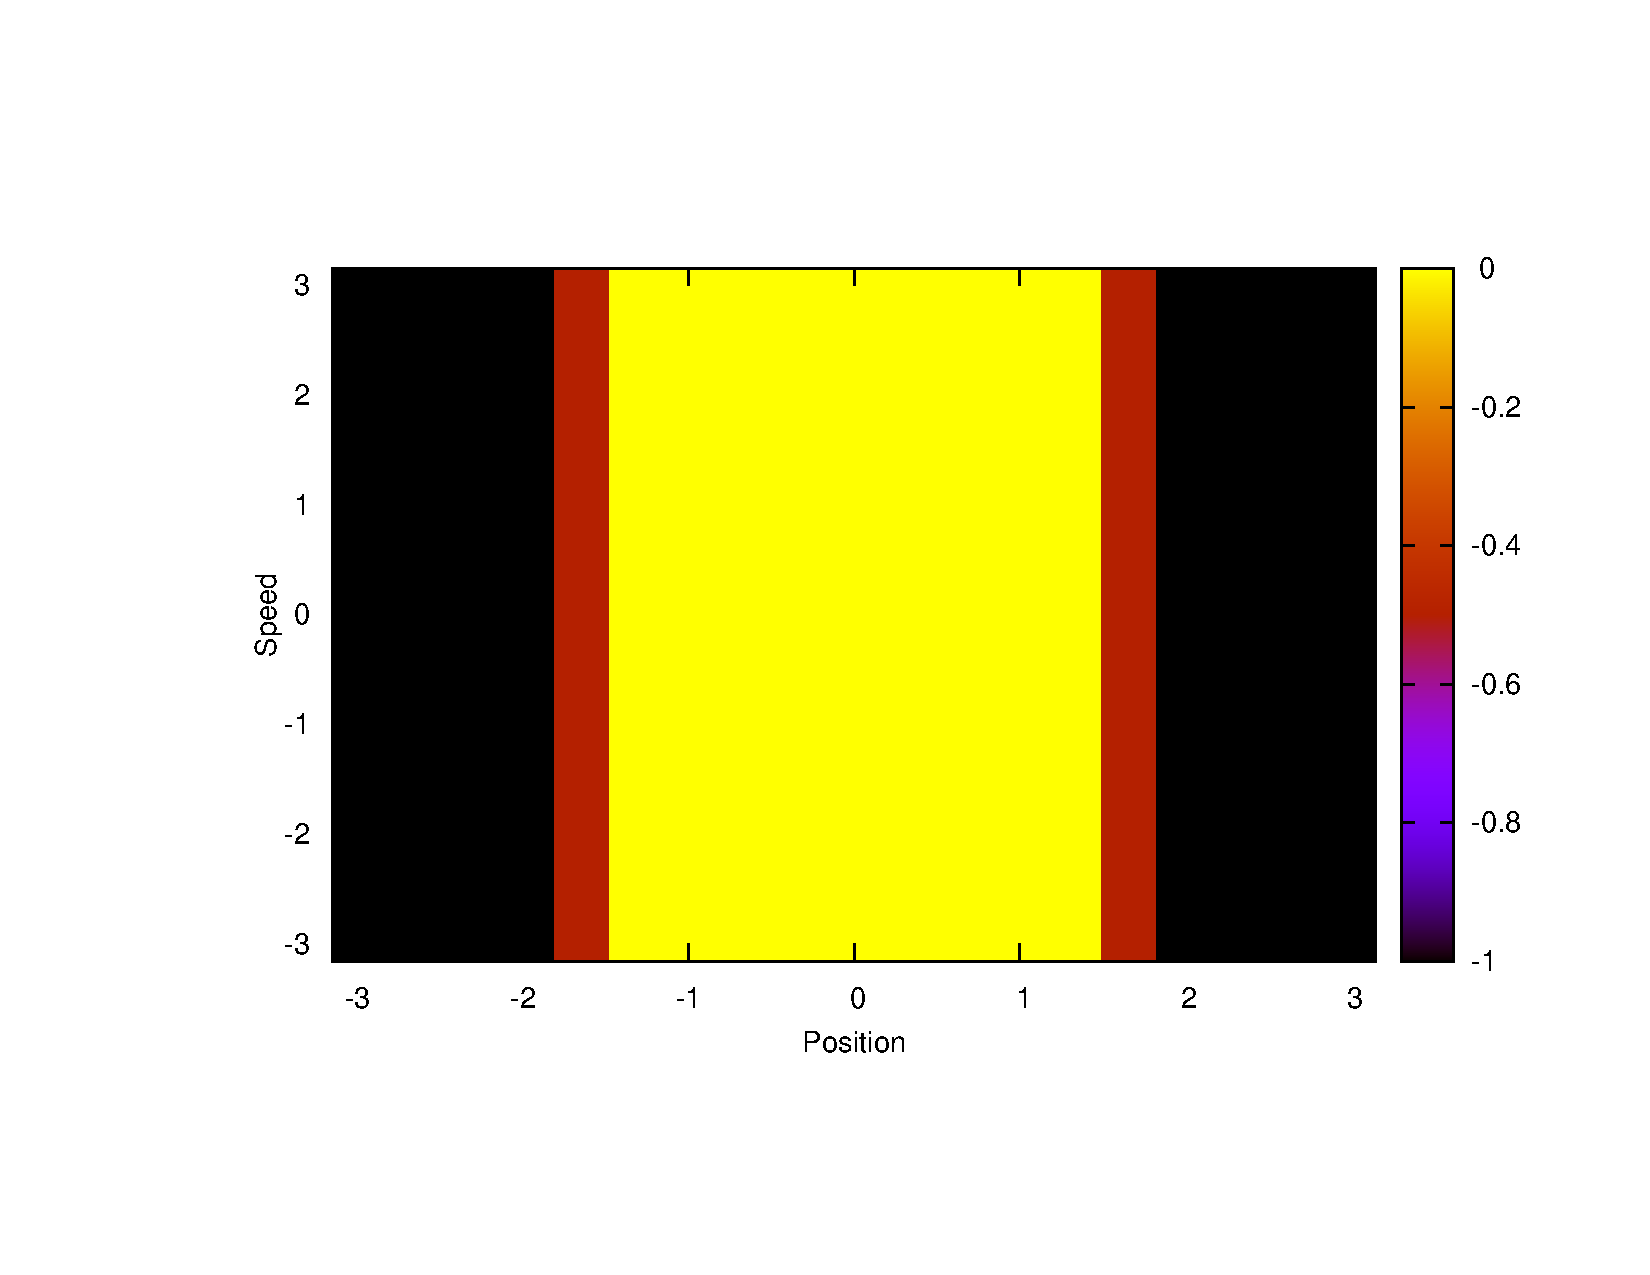
\includegraphics[width=1.2\linewidth]{LAFEM_Exp3_true_R.pdf}}
  \centerline{(a) Récompense de l'expert}%\medskip
\end{minipage}
\hfill
\begin{minipage}[b]{.5\linewidth}
  \centering
  \centerline{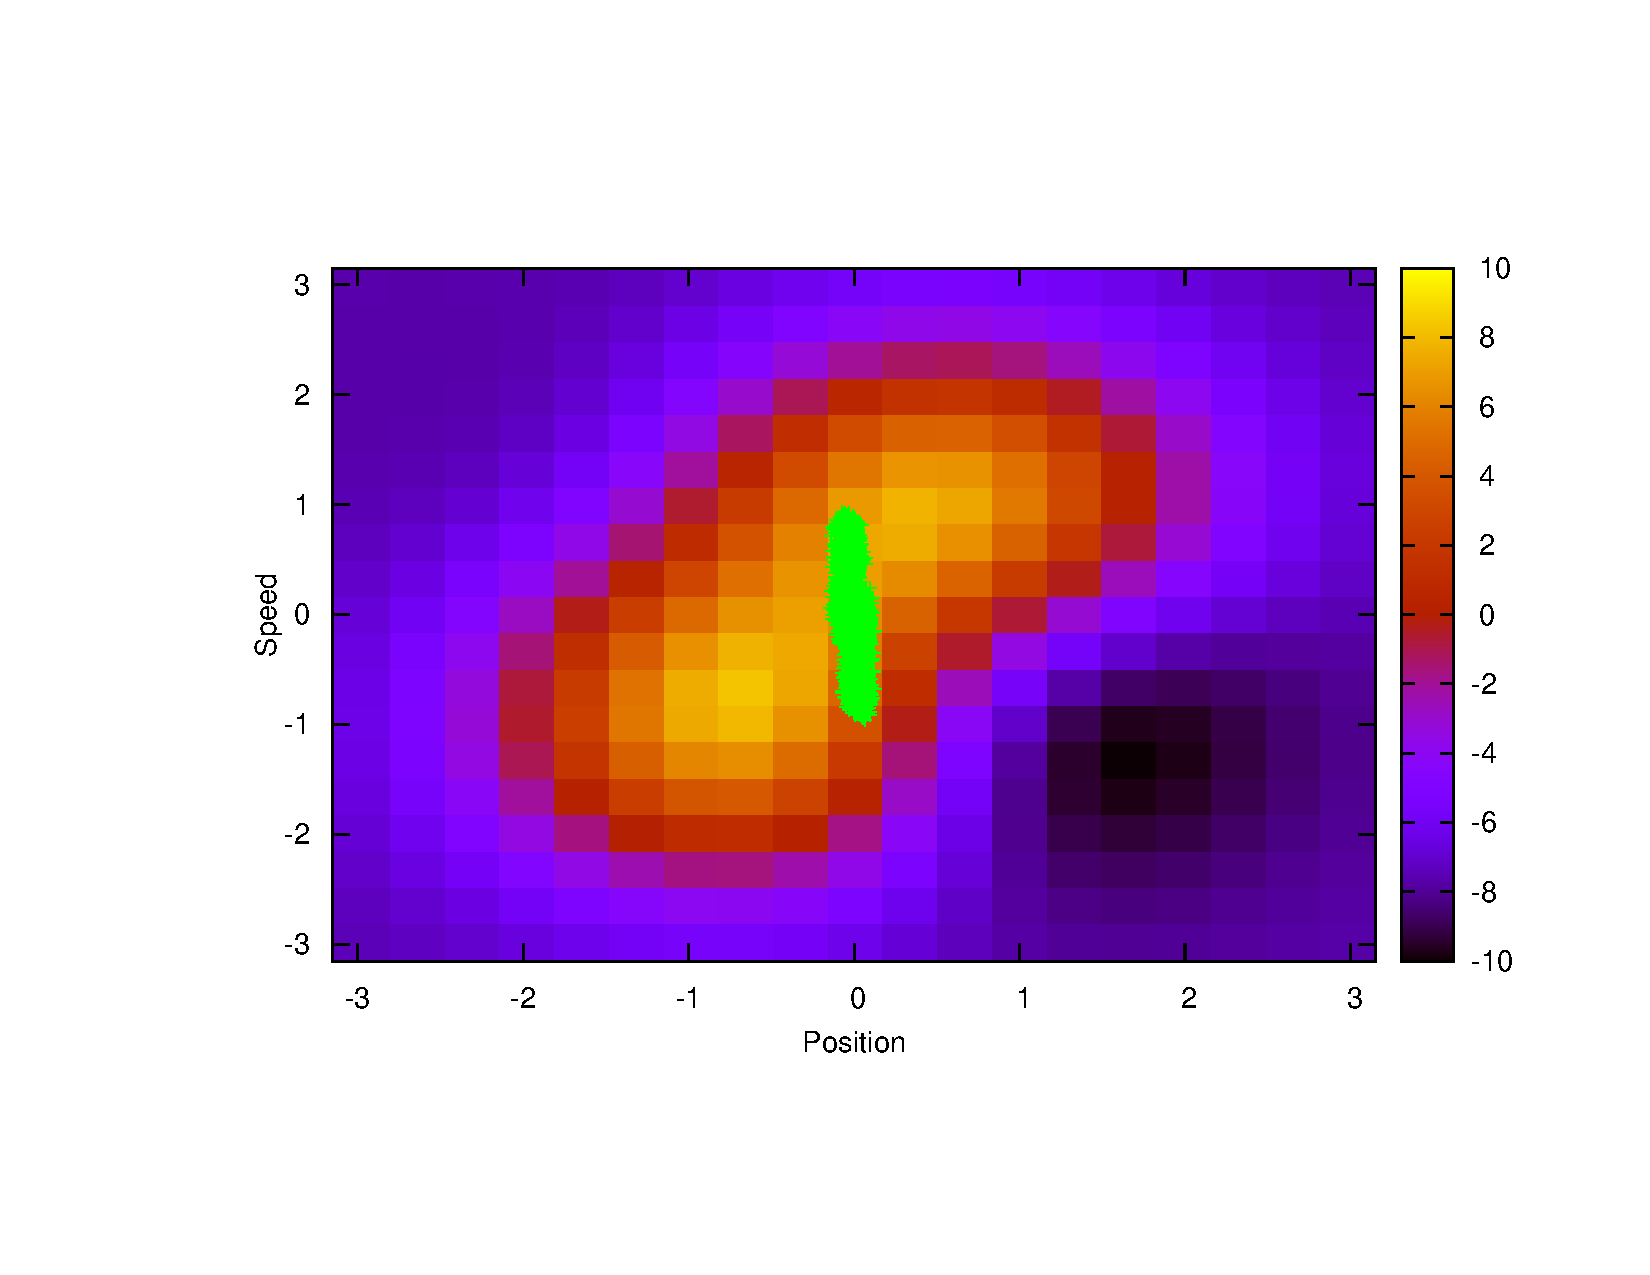
\includegraphics[width=1.2\linewidth]{LAFEM_Exp3_lafem_R.pdf}}
  \centerline{(b) Récompense trouvée}%\medskip
\end{minipage}
\begin{minipage}[b]{.5\linewidth}
  \centering
  \centerline{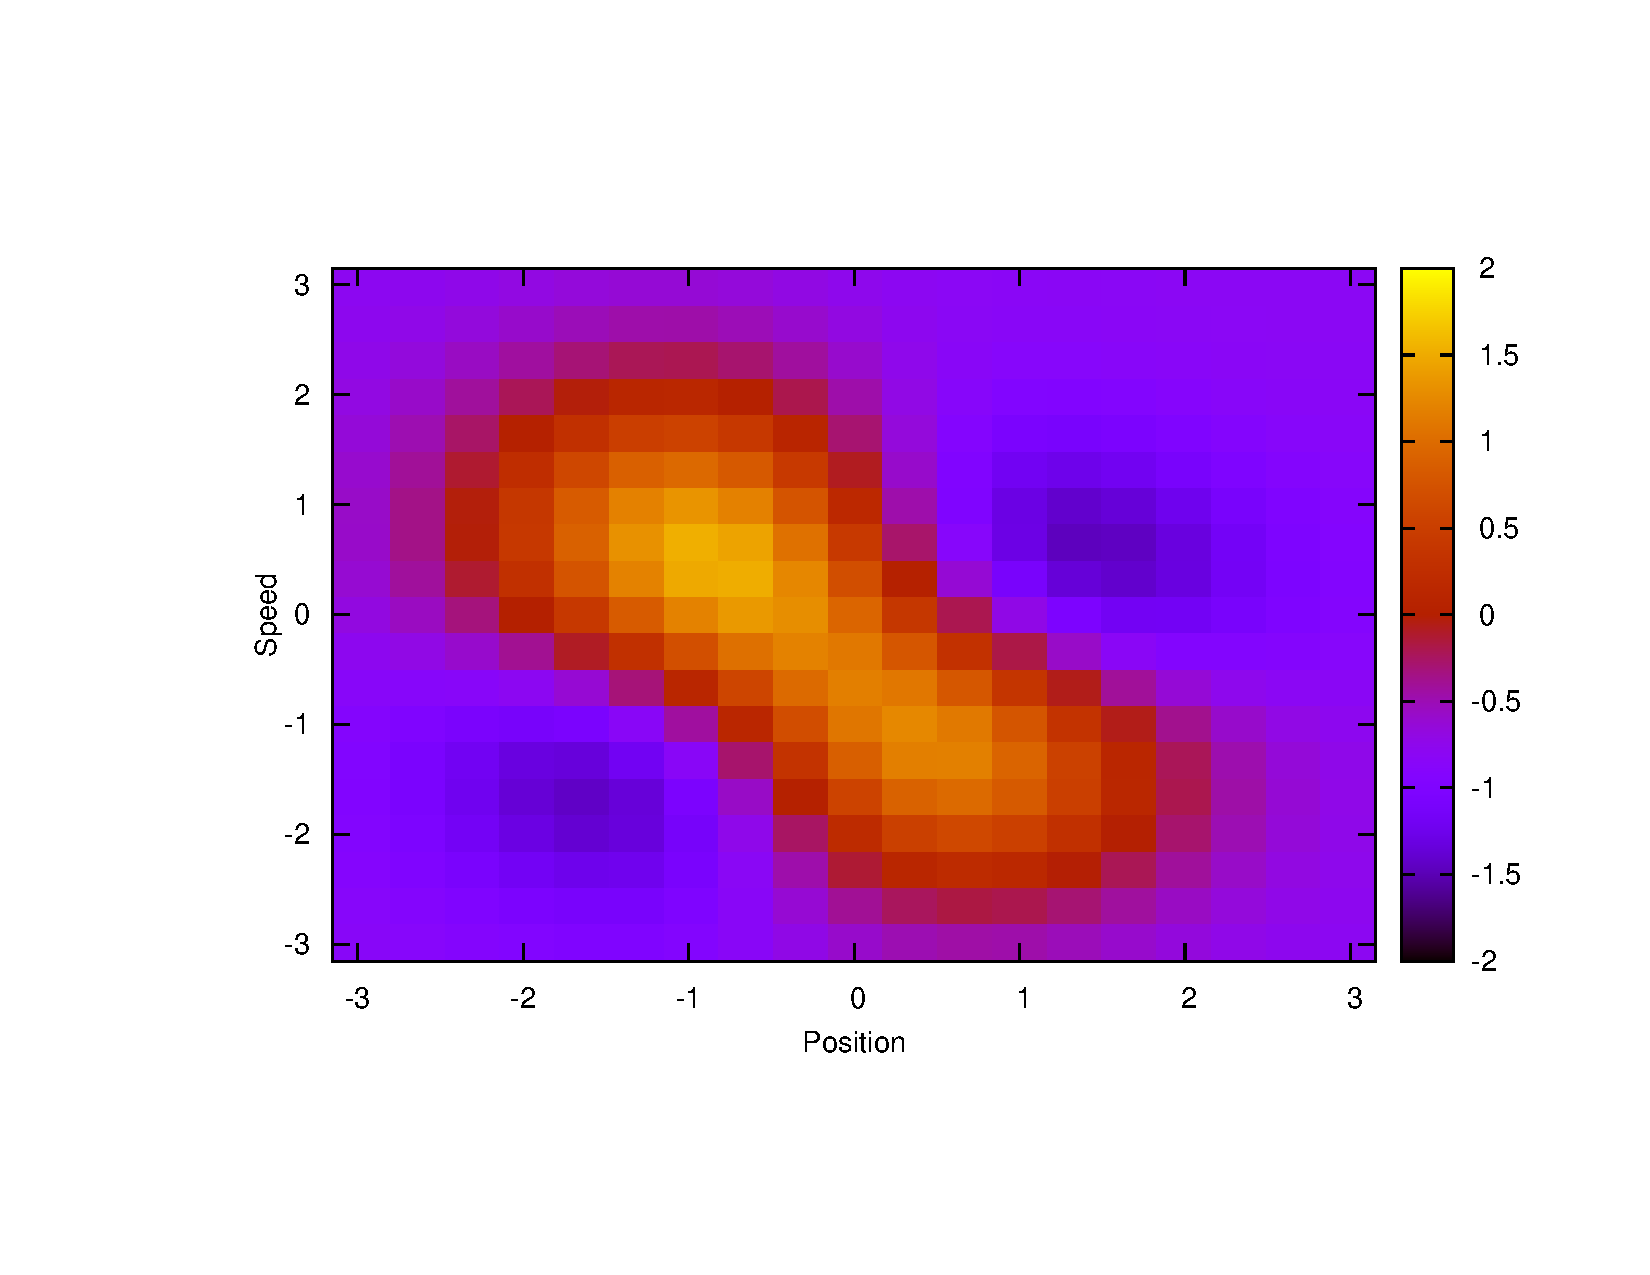
\includegraphics[width=1.2\linewidth]{LAFEM_Exp3_Vexpert.pdf}}
  \centerline{(c) Fonction de valeur de l'expert}%\medskip
\end{minipage}
\hfill
\begin{minipage}[b]{.5\linewidth}
  \centering
  \centerline{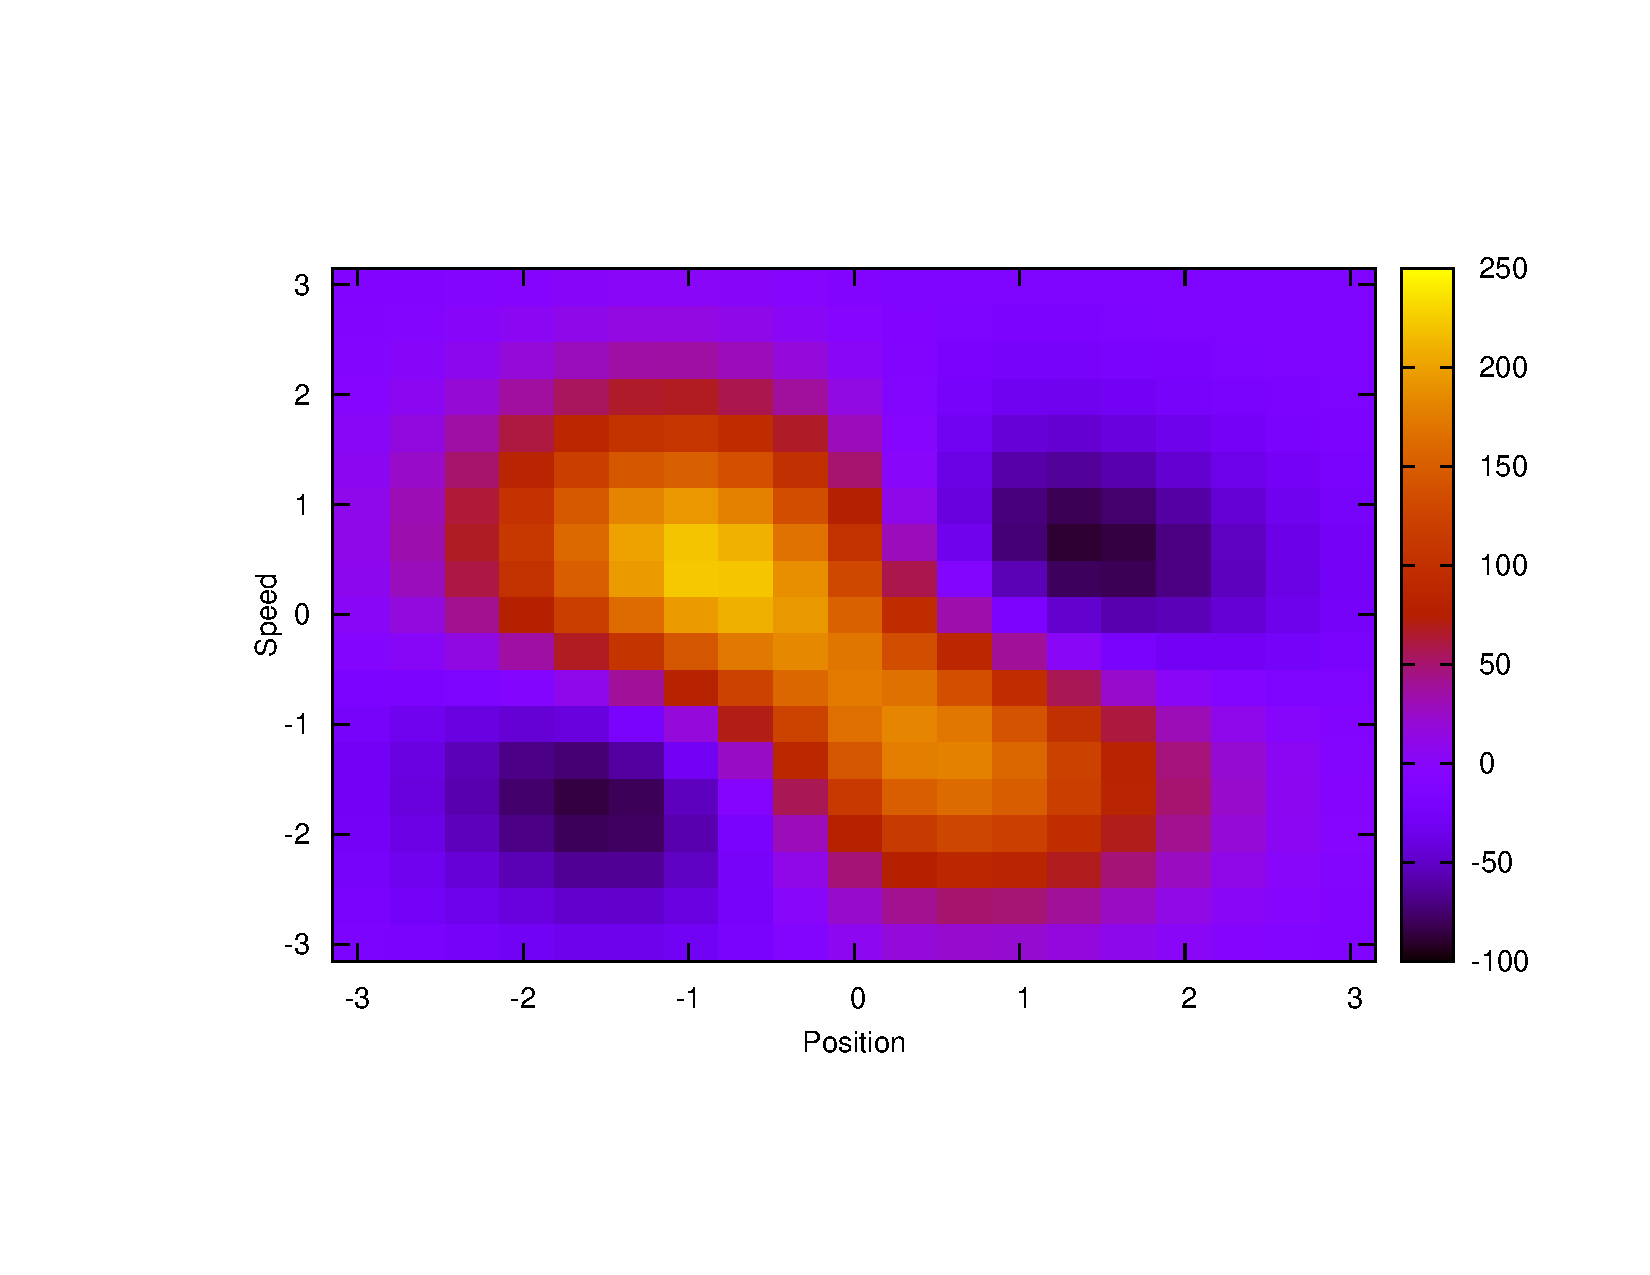
\includegraphics[width=1.2\linewidth]{LAFEM_Exp3_Vagent.pdf}}
  \centerline{(d) Fonction de valeur de l'agent}%\medskip
\end{minipage}
%
\caption{Résultats fournis par notre algorithme.}
\label{onlyFig.fig}
%
\vspace{-5pt}
\end{figure}

Afin d'étudier le comportement de notre algorithme, nous avons fait générer à l'expert une base de données $D_E$ de transitions contenant 10 trajectoires de 300 transitions chacune. La fonction $l$ fut définie sur les états présents dans $D_E$ telle que $l(s,a) = 0$ si $a=\pi_E(s)$, $1$ sinon. Le pas de temps est constant à $\alpha_t = 0.1$ et le nombre d'itérations est de $T=20$. Le vecteur initial $\theta_0$ fut fixé à $[-1...-1]^T$, la récompense étant paramétrée à l'aide du vecteur d'attribut $\psi: S \rightarrow \mathbb{R}^p$ correspondant au mélange de gaussiennes défini dans \cite{lagoudakis2003least}. Pour l'approximation de l'attribut vectoriel moyen de l'expert, c'est l'algorithme LSTD$\mu$ qui fut employé.\\


Si la fonction de récompense trouvée par LAFEM (figure \ref{onlyFig.fig} (b)) diffère de celle fournie à l'expert (figure \ref{onlyFig.fig} (a)) on constate en revanche que les fonctions de valeurs sont très similaires (figures \ref{onlyFig.fig} (c) et \ref{onlyFig.fig} (d)). Cela est une illustration du fait que le problème de l'ARI est mal posé en ceci qu'il n'y a pas qu'une seule récompense pouvant expliquer une politique.\\

Avec le nombre d'échantillons fournis par l'expert (3000 en 10 trajectoires de 300 transitions chacune), l'agent parvient systématiquement à maintenir le pendule en équilibre durant 5 minutes, ce qui est notre critère de réussite.\\

Deux éléments méritent d'être notés. Tout d'abord la faible couverture de l'espace d'état offerte par les échantillons de l'expert. Ceux-ci sont portés en vert sur la Figure \ref{onlyFig.fig} (b) et l'on constate qu'ils n'occupent qu'une toute petite partie de l'espace: celle dans laquelle le pendule est proche de la verticale. En l'absence de données dans le reste de l'espace d'état il n'est pas possible de pouvoir y inférer avec certitude la récompense. Le second point à noter est que la "vraie" récompense ne se trouve pas dans l'espace d'hypothèse que notre algorithme explore, en effet les attributs vectoriels utilisés ne peuvent qu'approximer la fonction de récompense utilisée sans l'atteindre. Malgré ces deux difficultés, notre algorithme parvient, comme nous l'avons dit, à extraire une récompense qui permet à un agent d'obtenir des performances similaires à celles de l'expert. Le lecteur attentif aura noté la différence d'amplitude des fonctions de valeur Fig. \ref{onlyFig.fig} Cela n'a aucune importance, une dilatation laissant la politique optimale invariante.
\section{Conclusion}

L'algorithme présenté dans cette contribution lève les problèmes les plus contraignants de l'apprentissage par renforcement inverse. En rendant la résolution du problème inverse indépendante de celle du problème direct, nous sommes en mesure d'inférer une récompense cohérente avec le comportement d'un expert en mode purement \emph{batch}.\\

Comme nous l'avons illustré, les échantillons nécessaires à la réussite de notre algorithmes sont faciles à recueillir. Une simple trace de l'expert, même si elle ne couvre qu'une petite partie de l'espace d'état, suffit à inférer une récompense. Cette récompense, description compacte de la tâche effectuée par l'expert, peut alors être optimisée par un agent dont les capacités diffèrent de celles de l'expert. On rentre dans le cadre du \emph{transfer learning}.\\

L'estimation de $mu_E$ est centrale dans notre approche. Nous disposons d'un algorithme efficace avec LSTD$\mu$, mais qui présente cependant les mêmes inconvénients que les algorithmes d'estimation d'une fonction de valeur. L'axe d'étude que nous envisageons d'explorer serait de ne plus passer par l'attribut vectoriel moyen en trouvant le moyen d'introduire autrment la structure du PDM dans la démarche de classification que nous avons adoptée. Des tests empiriques sur des problèmes plus comlpexes sont également envisagés.
%
% Bibliographie
%
\bibliography{Biblio}
\bibliographystyle{icml2012}
\end{document}

